This paper investigates the advantages and disadvantages of monolithic source code repositories compared to multi-repository systems through a case study conducted at Google. Using a mixed-methods approach that combines a large-scale survey of software engineers with analysis of developer tool logs, the study explores how repository structure influences developer experience, productivity, and code management. The results show that engineers generally prefer the monolithic repository model due to its high visibility across the entire codebase, which enables easier discovery of reusable APIs, access to example implementations, and streamlined dependency management. The ability to update dependencies and propagate API changes across the codebase further supports development efficiency.

However, the study also identifies important trade-offs between monolithic and multi-repository systems. While monolithic repositories provide centralized tooling, consistent development practices, and easier code reuse, multi-repository environments offer greater flexibility in selecting toolchains and managing stable, versioned dependencies. Engineers also associate multi-repo systems with improved build performance and reduced complexity due to smaller codebases. Overall, the findings highlight that the choice between repository models involves balancing visibility, standardization, and dependency management against flexibility, stability, and development autonomy.

\section{Motivation}

Modern software organizations produce extremely large and complex codebases, often composed of numerous projects that depend on shared libraries and frameworks. As the number of interdependencies between components grows, managing these relationships becomes increasingly important for maintaining development velocity and software quality. Organizations must therefore carefully choose how to structure and manage their source code repositories. A key architectural decision is whether to maintain a monolithic repository, where all projects reside in a single shared codebase, or a multi-repository system, where each project is stored in its own repository. Large technology companies such as Facebook, Google, and Microsoft have adopted monolithic repository models at scale, yet there has been relatively little empirical research examining the trade-offs between these repository structures \cite{goode2014scaling,harry2017scaling,potvin2016google}. Understanding the implications of these different repository strategies is essential for organizations seeking to support large-scale collaborative software development.

Another important motivation for the study arises from the uncertainty surrounding how developers actually benefit from the characteristics of monolithic repositories. Proponents of monolithic repositories argue that broad visibility into the entire codebase allows developers to understand APIs more effectively, discover reusable components, and coordinate changes across dependent systems. At the same time, critics suggest that such large codebases may overwhelm developers with irrelevant information and reduce flexibility in choosing tools and development practices. Prior research on developer workflows has shown that developers frequently rely on searching and exploring code to understand APIs and system behavior \cite{sadowski2015developers}. However, it remains unclear whether developers working in monolithic repositories genuinely exploit these capabilities in practice or whether the benefits are primarily perceived rather than realized. Investigating developer perceptions alongside actual usage behavior provides an opportunity to better understand the real impact of repository structure on development practices.

\begin{figure}[H]
    \centering
    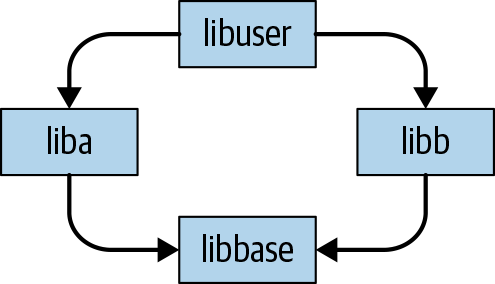
\includegraphics[width=0.45\textwidth]{diamond_dependency.png}
    \caption{The diamond dependency problem in multi-repository systems, where two projects depend on different versions of the same library, leading to potential conflicts and coordination challenges.}
    \label{monolithic:fig:diamond_dependency}
\end{figure}

The study is also motivated by long-standing challenges related to dependency management and collaboration in large software systems. In multi-repository environments, dependencies between projects are typically versioned and maintained independently, which can lead to problems such as version skew and the well-known “diamond dependency” (Figure \ref{monolithic:fig:diamond_dependency}) issue in dependency graphs \cite{florisson2017packages}. Managing these dependencies often requires significant coordination between teams and careful communication about changes to shared components. Prior research has shown that developers frequently rely on communication channels to coordinate dependency updates and manage changes across components \cite{desouza2008empirical}. Monolithic repositories offer an alternative approach in which dependencies are centralized and updated simultaneously across projects, potentially eliminating certain coordination challenges. Exploring whether this centralized model improves development practices provides an important motivation for empirically studying the trade-offs between repository models.

\subsection{Monolithic Repositories}

A monolithic repository (often referred to as a monorepo) is a source code management model in which the code for many projects within an organization is stored in a single, centralized repository. In this model, engineers typically have broad visibility into the entire codebase and interact with a shared set of tools for building, testing, browsing, and reviewing code. Large technology organizations have adopted this model to support large-scale development across multiple teams and products, demonstrating that a single repository can successfully manage extremely large codebases and thousands of developers \cite{potvin2016google}.

Monolithic repositories are characterized by several key features:
\begin{enumerate}
    \item \textbf{Centralization} All source code for multiple projects is stored within a single shared repository rather than being distributed across multiple repositories.
    \item \textbf{Visibility} Engineers across the organization can search, browse, and read code from any project in the repository, enabling easier discovery of APIs and reusable components.
    \item \textbf{Synchronization} Development typically follows a trunk-based workflow, where developers commit changes directly to the main branch of the repository.
    \item \textbf{Completeness} Projects rely on dependencies that are also stored within the same repository, meaning builds can be performed using code contained entirely within the repository without external versioned packages.
    \item \textbf{Standardization} Developers use a shared and consistent set of tools for activities such as building, testing, code browsing, and code review, ensuring uniform development practices across the organization.
\end{enumerate}

In contrast to monolithic repositories, multi-repository systems store projects in separate repositories, often leading to versioned dependencies and independent development workflows. While such systems provide greater flexibility in choosing tools and development practices, they can introduce challenges such as version skew and complex dependency relationships between projects. Monolithic repositories attempt to address these challenges by consolidating dependencies and development workflows within a single environment, enabling consistent tooling and easier coordination across teams.

\section{Methodology}
To investigate the advantages and disadvantages of monolithic repositories compared with multi repository systems, the study employs a mixed-methods case study within a large organization using a monolithic repository. The methodology combines two primary approaches. First, the researchers conducted a large-scale survey of software engineers to understand their perceptions, preferences, and experiences working with both monolithic and multi-repo environments. Second, they performed a quantitative analysis of developer tool logs to observe how engineers actually interact with the codebase, such as how frequently they view or modify code outside their immediate project. By combining perception-based survey data with behavioral log analysis, the study aims to validate whether the reported benefits of monolithic repositories are reflected in real developer activity.

\subsection{Assumptions}

The methodology is built upon several assumptions derived from prior internal observations about developer workflows and tooling. These assumptions guided both the design of the survey and the subsequent log analysis.

One key assumption is that \uline{developer tools strongly influence engineers' preferences for a particular repository model}. Internal surveys had consistently shown that the organization's development tools - such as code browsing, building, testing, and review systems - receive very high satisfaction ratings from engineers. Because of this, there was a concern that developers might rate the monolithic repository highly not because of the repository structure itself, but because of the quality of the associated tools. To address this potential bias, \uline{the survey design included questions that attempted to isolate the influence of tooling by asking participants to compare repository models under the assumption that tooling would remain constant}. This approach was intended to distinguish satisfaction with the repository model from satisfaction with the development tools.

A second assumption concerns the importance of code visibility within a monolithic repository. \textit{Developers often claim that the ability to search and explore the entire codebase is critical for productivity}, enabling them to understand APIs, locate examples of usage, and identify reusable components. However, the researchers were uncertain whether engineers truly make frequent use of this capability or whether its perceived importance stems mainly from the theoretical benefit of having access to all code. To investigate this, the study incorporated log analysis to measure actual developer interactions with the codebase. \uline{The logs allowed the researchers to determine how often engineers view or edit code outside their own teams or projects}, thereby validating whether the visibility advantage is actively utilized in practice.

A third assumption relates to the potential complexity of very large codebases. Prior internal surveys suggested that the massive scale of the organization's monolithic repository could overwhelm engineers due to the size and complexity of the codebase. \textit{Developers had previously reported concerns that navigating such a large repository might introduce cognitive overhead or make it difficult to identify relevant components}. The researchers therefore expected complexity to emerge as a significant theme when comparing monolithic and multi-repository systems. At the same time, they sought to understand whether these challenges outweigh the potential benefits of visibility, centralized dependency management, and standardized tooling.

\subsection{Survey Methodology}

To understand developers' perceptions of monolithic repositories and compare them with experiences in multi-repository environments, the study conducted a large-scale survey of software engineers within the organization. \textbf{The researchers randomly selected 1,902 engineers from a population of approximately 23,000 software engineers. To ensure participants had sufficient familiarity with the repository and development tools, the sample was restricted to engineers who had worked at the company for at least three months, had committed code to the repository in the previous six months, and had spent an average of at least five hours per week using developer tools}. The survey invitation followed established best practices from prior software engineering survey research to maximize participation, and reminder emails were sent to participants who had not completed the survey within the first 24 hours \cite{smith2013improving}. Ultimately, 869 engineers completed the survey, resulting in a response rate of approximately 46\%.

The survey was structured into three blocks of questions, with certain sections shown only to participants who had relevant prior experience.

\begin{enumerate}
    \item The first block was presented to all respondents and focused on overall satisfaction with the organization's monolithic repository, as well as perceptions of how the ability to search or edit code across the repository affects development velocity and code quality. It also collected background information about participants' prior experiences with different types of development environments, such as multi-repository corporate systems or open-source projects.
    \item The second block was shown only to engineers who had previously worked with multi-repository codebases. These questions asked participants to compare their prior experiences with the organization's monolithic repository, identify benefits of each approach, and indicate which model they preferred.
    \item The third block targeted engineers with open-source development experience and asked similar comparative questions regarding open-source repositories and the monolithic repository.
\end{enumerate}

In addition to quantitative rating questions, \textbf{the survey included free-response questions to capture developers' reasoning and motivations behind their preferences. The researchers analyzed these responses using an open coding methodology, in which responses were categorized into thematic tags}. Initially, common responses were identified and assigned labels representing recurring themes. The remaining responses were then collaboratively coded by multiple researchers to ensure consistent interpretation. Some responses were assigned multiple tags when they addressed several themes simultaneously. Disagreements between coders were resolved through discussion and re-examination of the responses, and the tagging process was refined as new themes emerged. \textit{The resulting coded data allowed the researchers to identify patterns in developer perceptions and quantify the most frequently cited advantages and disadvantages of different repository models.}

\subsection{Log Based Methodology}
In addition to the survey, the study conducted a quantitative analysis of developer tool logs to examine how engineers actually interact with the monolithic repository. \textbf{While the survey captured developers' perceptions and preferences, the log analysis provided behavioral evidence regarding how the repository is used in practice. The goal was to determine whether engineers truly take advantage of the visibility and cross-project access enabled by a monolithic repository}, particularly by measuring how frequently developers view or modify code outside their immediate areas of responsibility.

The analysis focused on two types of logs generated by internal developer tools.
\begin{enumerate}
    \item \textbf{Code Browsing Logs} which recorded every instance in which an engineer viewed a source file using the organization's web-based code browsing tool. This tool is commonly used by developers to search and explore the codebase, particularly because traditional local development environments have difficulty indexing and navigating extremely large repositories.
    \item \textbf{Code Commit Logs} which captured the changes engineers submitted to the repository. By examining both file views and code commits, the researchers were able to study both passive interactions (such as reading code) and active contributions (such as modifying code).
\end{enumerate}
\textbf{To determine whether interactions occurred outside a developer's primary project area, the researchers analyzed activity at the level of Product Areas (PAs) within the organization. The company's engineering structure contained twelve such areas, and engineers were assigned to one of them during each week of the study period}. Any interaction with code belonging to a different product area was therefore considered likely to represent cross-project activity. To enable this analysis, the researchers created mappings between engineers and product areas, as well as between source files and product areas. File ownership information was derived from project metadata that identified which directories belonged to particular projects and product areas. When metadata was incomplete or ambiguous, the researchers inferred ownership by examining code review records, since reviewers were typically the owners responsible for the corresponding directories.

After establishing these mappings, \textbf{the researchers calculated the percentage of each engineer's file views and commits that occurred outside their assigned product area. These percentages were computed weekly for each engineer over a one-year period and then averaged across time}. The resulting distribution allowed the researchers to quantify how frequently developers interacted with code outside their primary domain. This analysis provided empirical evidence about the extent to which engineers utilize the visibility and cross-project collaboration capabilities that monolithic repositories are designed to support.

\subsection{Threats to Validity}
The authors discuss several threats to validity that may affect the interpretation of the study's results. One potential issue is selection bias in the survey population. \textbf{Developers may choose to work at organizations whose repository structures align with their personal preferences}. For example, engineers who prefer multi-repository environments may choose companies that use such systems, while those comfortable with monolithic repositories may prefer organizations structured around that model. \textbf{As a result, the survey responses may reflect the preferences of developers who are already accustomed to a monolithic repository environment}. Additionally, although the survey achieved a relatively high response rate of 46\%, there is still a possibility of nonresponse bias, where the opinions of engineers who did not participate could differ from those who responded.

Another potential threat arises from the influence of internal developer tools. \textbf{Engineers might have rated the monolithic repository positively not because of the repository structure itself, but because of the quality of the tools used to interact with it. Since the organization has invested heavily in specialized tools for code browsing, building, testing, and reviewing code, these tools may strongly shape developer satisfaction}. To mitigate this confounding factor, the survey included questions designed to separate preferences for repository structure from preferences for tooling by asking participants to compare repository models under the assumption that the same tools would be available in both environments.

The survey design may also be affected by priming effects. Certain questions asked participants to consider how the ability to search and edit the entire codebase influences development velocity and code quality. These questions might have influenced how participants later evaluated the advantages of monolithic repositories, potentially encouraging them to think more about visibility and productivity benefits when responding to later survey questions. Such priming could bias responses toward emphasizing certain perceived benefits.

Another limitation relates to the subjectivity of the qualitative analysis process. The researchers used an open-coding methodology to categorize free-response survey answers into thematic groups. While multiple researchers collaborated during the coding process to reduce individual bias and disagreements were resolved through discussion, qualitative coding inherently involves interpretation. Therefore, the resulting themes and categorizations may not represent the only possible interpretation of the responses.

Finally, there are potential validity threats in the log analysis methodology, particularly in the heuristic used to map source files and developers to product areas. Although most directories were mapped using project metadata or code review records, some directories lacked clear ownership information or had multiple possible owners. In such cases, the researchers relied on majority ownership assumptions or excluded certain directories from the analysis. These approximations may introduce small inaccuracies in determining whether interactions occurred inside or outside a developer's primary product area, though the authors report that the overall impact of such inaccuracies is minimal.

\section{Results and Key Findings}
\subsection{Results}
The results of the study combine insights from the survey responses and the developer tool log analysis to understand how engineers perceive and use a monolithic repository. The findings reveal both strong preferences for the monolithic model and clear trade-offs compared with multi-repository environments. \textbf{Overall, the results suggest that the advantages of visibility, code reuse, and centralized dependency management are major drivers behind developer satisfaction with monolithic repositories}.

From the survey responses, the study first analyzed the background of the 869 engineers who participated. A large portion of respondents had diverse development experiences, including starting new codebases from scratch, working with corporate multi-repository environments, and contributing to open-source projects. This diversity allowed the researchers to compare perceptions of the monolithic repository against alternative repository models based on real developer experience. The survey also examined how developers perceived the impact of repository features on development velocity and code quality. \textbf{The majority of participants reported that the ability to search across the entire codebase is highly important for both productivity and code quality. In contrast, opinions were more mixed regarding the importance of the ability to edit code across projects, suggesting that visibility of code may be more valuable than cross-project modification capabilities in everyday development tasks}.

The log analysis results provided behavioral evidence supporting the importance of code visibility in a monolithic repository. The analysis measured how often engineers interacted with code belonging to different product areas within the organization. \textbf{The results showed that developers frequently view code outside their own teams or projects. For instance, the median value indicated that more than a quarter of code views by engineers involved files from outside their assigned product area. Similarly, a significant portion of engineers committed changes to code belonging to other product areas}. These findings demonstrate that developers actively explore and interact with code across the organization, confirming that the visibility provided by a monolithic repository is widely utilized in practice.

To further understand the nature of cross-project interactions, the researchers examined whether developers primarily accessed widely used shared libraries or whether they explored other parts of the codebase as well. The analysis excluded highly common files such as widely used libraries, build configuration files, and service interface definitions. \textbf{Even after excluding these commonly accessed files, the patterns of cross-project interactions remained largely unchanged. This indicates that developers are not only accessing well-known shared libraries but are also exploring a wide variety of code throughout the repository}, often to understand implementations or find examples of API usage.

\subsubsection{Participants with Corporate Multi-Repo Codebase Experience}

A significant portion of the survey participants reported prior experience working in organizations that used multiple repositories for managing source code. \textit{Out of the 869 engineers who completed the survey, 379 participants indicated that they had previously worked with a corporate multi-repository codebase}. This subgroup provided an important basis for comparing developer experiences between monolithic repositories and multi-repository environments, since these participants had direct exposure to both development models. Their responses allowed the researchers to examine satisfaction levels, preferences, and perceived advantages of each repository structure based on real-world experience rather than hypothetical comparisons.

The study first compared developer satisfaction with the current monolithic repository against satisfaction with their previous multi-repository environments. \textbf{The results showed a clear difference in overall satisfaction levels. While engineers reported generally high satisfaction with the monolithic repository used in the organization, their satisfaction with previous multi-repository systems was considerably more mixed}. This suggests that many developers found the monolithic repository to provide a more consistent or supportive development environment compared with the multi-repository systems they had previously used.

The survey also asked participants to directly compare the two repository models and indicate which they preferred. Among the respondents with multi-repository experience, a large majority expressed a preference for the monolithic repository, while only a small number preferred their previous multi-repository environments and some participants reported no strong preference. When participants explained the reasons behind their choices, several recurring themes emerged. \textbf{The most frequently cited motivations for preferring the monolithic repository included improved code reuse, the ability to search and view the entire codebase, and simplified dependency management}. These factors enable developers to easily discover APIs, examine implementation examples, and integrate existing components without needing to locate code across separate repositories.

Despite the strong preference for the monolithic repository, participants also identified several advantages of multi-repository systems. \textbf{One commonly cited benefit was the ability to maintain stable and versioned dependencies, which allows projects to control when updates are adopted rather than automatically receiving changes from other parts of the codebase. Developers also associated multi-repository systems with improved build performance, since smaller repositories often require fewer dependencies to be compiled}. Additionally, multi-repository environments allow teams greater flexibility in selecting development tools and configuring their own workflows, which some developers considered beneficial for project autonomy.

The survey further explored how engineers would prefer to structure the organization's codebase if given the option. Even when asked to assume that developer tools would remain the same in both scenarios, most participants still preferred maintaining the existing monolithic repository structure rather than splitting the codebase into multiple repositories. However, a minority of respondents expressed interest in a multi-repository model primarily due to concerns about build times and the stability of dependencies. These responses highlight the inherent trade-offs between centralized coordination and flexibility in repository design.

Overall, the responses from developers with corporate multi-repository experience indicate that while both repository models have advantages, engineers in this study generally favored the monolithic repository because of its ability to improve visibility, facilitate code reuse, and simplify dependency management across a large organization.

\subsubsection{Participants with Open-Source Experience}

The survey also included a subgroup of engineers who had prior experience contributing to open-source projects. \textit{Out of the 869 survey respondents, 337 participants reported working with open-source repositories. These repositories are particularly relevant for comparison because they typically provide broad visibility into source code, similar to monolithic repositories, while still following a multi-repository structure}. By analyzing the responses of developers familiar with open-source development, the study aimed to understand how engineers perceive the differences between open-source repository environments and the organization's monolithic repository.

Participants in this group were asked to compare their experience with their most recent open-source codebase and the monolithic repository used within the organization. The results showed that most respondents preferred the monolithic repository, while a smaller number favored the open-source repository environment and some participants reported no strong preference. \textbf{These responses indicate that although open-source repositories offer many advantages, developers in this study generally viewed the monolithic repository as providing a more efficient environment for large-scale collaborative development within an organization}.

Respondents were also asked to identify the benefits of working within the monolithic repository when compared with open-source codebases. \textbf{Many developers highlighted advantages such as the ability to easily search and explore the entire codebase, improved code reuse, and the availability of usage examples for APIs. Developers also cited the ease of updating dependencies and propagating changes across projects, as well as the presence of integrated development tools that support code browsing, testing, and collaboration}. These characteristics make it easier for engineers to understand how different parts of the system interact and to reuse existing components when implementing new features.

At the same time, respondents identified several advantages associated with open-source repositories. One commonly cited benefit was the strong sense of community and collaboration, where developers contribute to projects that are shared with a broader public audience. Participants appreciated the opportunity to share their work with the wider developer community and contribute to widely used software. Open-source environments were also associated with greater flexibility in tools and workflows, allowing developers to choose technologies and practices that best fit their projects. In addition, the typically smaller size of individual repositories in open-source development can reduce complexity and make projects easier to navigate.

Overall, the responses from developers with open-source experience highlight both similarities and differences between open-source and monolithic repository environments. While both models provide significant visibility into code, the monolithic repository offers stronger integration of tools, easier cross-project coordination, and improved opportunities for code reuse within a large organization. Conversely, open-source repositories emphasize community engagement, flexibility, and autonomy in development practices.

\subsection{Key Findings}
\paragraph{Visibility of the Codebase Improves Development Efficiency}

One of the most important findings of the study is that the visibility provided by a monolithic repository strongly benefits developers. Engineers reported that the ability to search and explore the entire codebase significantly improves development velocity and code quality. Developers frequently rely on this visibility to understand APIs, examine implementations, and locate reusable components. The log analysis confirmed that engineers regularly view code across different product areas, demonstrating that this visibility is actively used rather than simply perceived as beneficial.

\paragraph{Code Reuse and API Discovery Are Major Advantages}

Another key finding is that monolithic repositories facilitate code reuse and easier API discovery. Because all projects exist within a single repository, developers can quickly find examples of how APIs are used in other parts of the organization. This enables engineers to reuse existing functionality instead of reimplementing similar features. The visibility of implementation details and usage examples helps developers learn how to integrate APIs effectively and reduces the effort required to adopt shared libraries.

\paragraph{Centralized Dependency Management Simplifies Development}

The study found that monolithic repositories simplify dependency management across projects. In a monolithic system, dependencies are maintained within the same repository and typically use a single version at the repository head. This allows changes to libraries and APIs to propagate across the codebase more easily and reduces issues such as incompatible versions of the same dependency. Developers reported that this centralized approach eliminates many of the coordination challenges commonly found in multi-repository environments.

\paragraph{Trade-off Between Dependency Updates and Stability}

Despite the advantages of centralized dependency management, the study identifies a trade-off between automatic updates and dependency stability. While monolithic repositories allow developers to receive updates to dependencies automatically, this can sometimes cause disruptions if upstream changes introduce breaking modifications. In contrast, multi-repository systems allow projects to maintain versioned dependencies and update them only when they choose. This trade-off highlights the balance between ease of updates in monolithic repositories and stability in multi-repository environments.

\paragraph{Developer Tools Play a Critical Role}

The research also found that developer tools are a significant factor in developer satisfaction, sometimes even more influential than the repository structure itself. Engineers frequently cited internal tools—such as code browsing and review systems—as key reasons for preferring the monolithic repository environment. At the same time, developers working in open-source environments often valued industry-standard tools such as Git. This finding suggests that the effectiveness of repository models is closely tied to the quality of the tooling that supports them.

\paragraph{Tension Between Standardization and Flexibility}

The study highlights a tension between standardization and flexibility in repository design. Monolithic repositories enforce consistent development practices, standardized tooling, and shared coding styles across the organization. Many developers consider this consistency beneficial because it improves code quality and reduces confusion when working across projects. However, some developers prefer the flexibility offered by multi-repository environments, where teams can select their own tools, programming languages, and workflows based on the needs of their projects.

\paragraph{Managing Cognitive Load in Large Codebases}

Another key insight relates to developer cognitive load when working with large codebases. Some engineers believed that monolithic repositories reduce cognitive load because developers can easily search the codebase, find examples, and rely on consistent tools. Others argued that the large size of a monolithic repository can increase complexity and make it harder to navigate. In contrast, multi-repository systems reduce cognitive load by limiting the scope of the code developers must understand, as each repository is typically smaller and more focused.

\paragraph{Cross-Project Collaboration Is Common}

The log analysis revealed that cross-project interaction occurs frequently in a monolithic repository. Developers regularly view and modify code belonging to different product areas, indicating that engineers collaborate across team boundaries more often than expected. Importantly, this behavior persists even after excluding commonly accessed libraries, suggesting that developers actively explore diverse parts of the codebase rather than only interacting with widely used shared components.

\subsection{Implications}
\paragraph{Repository Visibility Supports Organizational Knowledge Sharing}
One implication highlighted by the study is that repository visibility can significantly improve knowledge sharing across an organization. When developers have access to the entire codebase, they can examine implementations, understand how APIs are used, and identify reusable components. This allows engineers to learn from existing solutions and reduces duplicated development effort. As a result, organizations adopting monolithic repositories may benefit from faster onboarding and improved collaboration across teams.

\paragraph{Centralized Dependency Management Reduces Coordination Overhead}
The findings suggest that centralized dependency management in monolithic repositories can simplify coordination between teams. Since all dependencies are maintained within the same repository and are typically updated together, developers can propagate changes to dependent systems more easily. This reduces the need for complex communication and version negotiation that often occurs in multi-repository environments when dependencies change. Consequently, organizations may experience smoother integration and maintenance of shared libraries.

\paragraph{Developer Tooling Is Critical to Repository Model Success}
Another implication from the study is that the effectiveness of any repository model depends heavily on the quality of the supporting development tools. Engineers in the study frequently cited developer tools—such as code browsing and review systems—as key factors influencing their satisfaction with the monolithic repository. This suggests that organizations considering large-scale repository models must invest in strong tooling infrastructure to ensure efficient navigation, building, and testing of large codebases.

\paragraph{Repository Design Should Align with Organizational Scale}
An additional implication is that repository structure should be chosen based on the scale and collaboration patterns of an organization. Large organizations with many interconnected projects may benefit from monolithic repositories because they enable cross-team collaboration and code reuse. In contrast, smaller organizations or independent teams may find multi-repository systems more suitable, as they provide flexibility and reduced complexity. This suggests that repository architecture decisions should consider organizational size, dependency structure, and development workflows.

\paragraph{Improved Tooling Could Mitigate Monorepo Complexity}
The study also implies that many challenges associated with monolithic repositories—such as navigating extremely large codebases—can potentially be mitigated through improved tooling. Advanced code search, dependency visualization, and automated refactoring tools could help developers navigate large repositories more effectively. By investing in such capabilities, organizations could preserve the benefits of repository visibility while minimizing the cognitive load associated with large codebases.

\paragraph{Hybrid Repository Models May Provide Balanced Trade-offs}
Finally, the results suggest that hybrid repository strategies may be worth exploring. While monolithic repositories provide strong visibility and centralized dependency management, multi-repository systems offer stability and flexibility. A hybrid approach—such as grouping related systems into larger repositories while keeping loosely connected projects separate—could allow organizations to balance the benefits of both models. Such approaches may help organizations tailor repository structures to the specific needs of their development ecosystem.

\section{Related Work}
Research on monolithic repositories is relatively limited because the widespread adoption of such repository structures in industry is a comparatively recent development. However, some prior work has explored the scale and rationale behind these repository models. For example, earlier discussions of large-scale codebase management describe how major technology companies store massive codebases within a single repository to support collaboration across thousands of developers and enable consistent development practices \cite{potvin2016google}. These industry experiences demonstrate that monolithic repositories can scale to extremely large codebases while enabling shared tooling and centralized development workflows.

Related work has also examined how developers interact with large codebases, particularly through code search and exploration tools. Studies investigating developer search behavior have shown that developers frequently rely on searching across large codebases to understand APIs, examine implementations, and debug issues \cite{sadowski2015developers}. These findings highlight the importance of visibility and code discovery in software development, supporting the idea that large repositories with comprehensive search capabilities can improve developer productivity. The results of the present study reinforce these observations by showing that engineers actively use repository-wide search and browsing capabilities.

Another relevant line of research focuses on version control systems and repository management practices. Early version control systems such as the Source Code Control System and the Revision Control System established foundational mechanisms for tracking code changes and managing collaboration in software projects \cite{rochkind1975sccs,tichy1985rcs}. Later work has explored the conceptual design and usability challenges of modern version control systems such as Git \cite{perez2013git,perez2016purposes}. While most traditional version control systems were designed around per-project repositories, these systems can also support monolithic repository structures with appropriate tooling and infrastructure.

The rise of distributed version control systems has also prompted research on the differences between centralized and distributed development models. Some studies examine how these systems influence collaboration, development workflows, and software changes in large projects \cite{brindescu2014impact,deAlwis2009why}. Although this research primarily focuses on centralized versus distributed version control, it provides insights into how repository organization and collaboration models affect development practices. These questions are related but orthogonal to the monolithic versus multi-repository debate explored in this paper.

Research on dependency management and coordination among developers is also closely related to repository structure. Prior empirical studies have shown that developers often rely on communication channels to coordinate changes to shared components and dependencies \cite{desouza2008empirical}. In multi-repository environments, teams must notify downstream projects about changes to shared libraries, which can introduce coordination overhead. Monolithic repositories attempt to address this challenge by centralizing dependencies and allowing updates to propagate across the codebase simultaneously.

Finally, a large body of work has examined open-source repositories and collaborative development ecosystems. Studies of platforms such as GitHub have analyzed collaboration patterns, programming language usage, and community dynamics in open-source projects \cite{kalliamvakou2014promises,vasilescu2016sky,ray2014languages}. While open-source repositories share certain characteristics with monolithic repositories—such as broad visibility into source code—they typically lack the centralized tooling and unified dependency management found in monolithic repository environments. These differences highlight the distinct trade-offs between open-source repository ecosystems and large organizational monolithic repositories.
